\documentclass{beamer}
\usetheme{Madrid}
\usecolortheme{default}

\usepackage{amsmath}
\usepackage{amsfonts}
\usepackage{amssymb}
\usepackage{graphicx}
\usepackage{booktabs}
\usepackage{algorithm}
\usepackage{algpseudocode}
\usepackage{tikz}
\usetikzlibrary{arrows,positioning,shapes.geometric}

\title[Triangular Arbitrage Optimization]{Triangular Arbitrage Optimization Using Linear Programming}
\subtitle{A Mathematical Approach to Cryptocurrency Trading}
\author{Financial Engineering Project}
\institute{University Course - Optimization Methods}
\date{\today}

\begin{document}

\frame{\titlepage}

\begin{frame}
\frametitle{Outline}
\tableofcontents
\end{frame}

\section{Introduction and Problem Definition}

\begin{frame}
\frametitle{What is Triangular Arbitrage?}
\begin{itemize}
    \item \textbf{Arbitrage}: Simultaneous purchase and sale of an asset to profit from price differences
    \item \textbf{Triangular Arbitrage}: Exploiting inconsistencies in exchange rates between three currencies
    \item \textbf{Example}: USD $\rightarrow$ BTC $\rightarrow$ ETH $\rightarrow$ USD
\end{itemize}

\vspace{0.5cm}

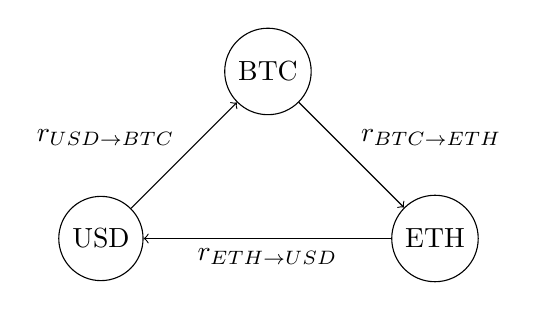
\begin{tikzpicture}[node distance=3cm, auto]
    \node[circle, draw] (USD) {USD};
    \node[circle, draw] (BTC) [above right of=USD] {BTC};
    \node[circle, draw] (ETH) [below right of=BTC] {ETH};
    
    \draw[->] (USD) to node {$r_{USD \rightarrow BTC}$} (BTC);
    \draw[->] (BTC) to node {$r_{BTC \rightarrow ETH}$} (ETH);
    \draw[->] (ETH) to node {$r_{ETH \rightarrow USD}$} (USD);
\end{tikzpicture}

\end{frame}

\begin{frame}
\frametitle{Mathematical Foundation}
For a triangular arbitrage opportunity to be profitable:

\begin{align}
r_{A \rightarrow B} \times r_{B \rightarrow C} \times r_{C \rightarrow A} > 1
\end{align}

Where:
\begin{itemize}
    \item $r_{A \rightarrow B}$ = exchange rate from currency A to currency B
    \item Net profit = $(r_{A \rightarrow B} \times r_{B \rightarrow C} \times r_{C \rightarrow A}) - 1$
\end{itemize}

\vspace{0.5cm}

\textbf{In practice, we must account for:}
\begin{itemize}
    \item Transaction fees
    \item Liquidity constraints
    \item Market impact
    \item Execution risk
\end{itemize}
\end{frame}

\begin{frame}
\frametitle{Problem Statement}
\textbf{Objective}: Maximize expected profit from multiple triangular arbitrage opportunities while respecting portfolio constraints.

\vspace{0.5cm}

\textbf{Given}:
\begin{itemize}
    \item Set of $n$ triangular arbitrage opportunities
    \item Portfolio constraints (initial balances, minimum holdings, risk tolerance)
    \item Market conditions (liquidity, transaction fees)
\end{itemize}

\vspace{0.5cm}

\textbf{Find}: Optimal allocation of capital across opportunities to maximize risk-adjusted returns.
\end{frame}

\section{Mathematical Model}

\begin{frame}
\frametitle{Decision Variables}
Let $x_i$ be the amount invested in arbitrage opportunity $i$, where $i = 1, 2, \ldots, n$.

\vspace{0.5cm}

Each opportunity $i$ is characterized by:
\begin{itemize}
    \item $p_i$: Expected profit rate
    \item $c_i$: Confidence score (reliability measure)
    \item $L_{i,j}$: Liquidity available for trading pair $j$ in opportunity $i$
    \item $f_{i,j}$: Transaction fee for trading pair $j$ in opportunity $i$
\end{itemize}
\end{frame}

\begin{frame}
\frametitle{Objective Function}
We maximize the risk-adjusted expected profit:

\begin{align}
\max \quad Z = \sum_{i=1}^{n} p_i \cdot c_i \cdot x_i
\end{align}

Where:
\begin{itemize}
    \item $p_i \cdot c_i$ represents the risk-adjusted profit rate
    \item Higher confidence scores weight more reliable opportunities
    \item Linear objective allows for efficient optimization
\end{itemize}
\end{frame}

\begin{frame}
\frametitle{Constraint Set: Portfolio Balance}
For each currency $k$, ensure we don't exceed available balances:

\begin{align}
\sum_{i \in S_k} x_i \leq B_k \quad \forall k
\end{align}

Where:
\begin{itemize}
    \item $S_k$ = set of opportunities requiring currency $k$ as initial investment
    \item $B_k$ = available balance of currency $k$
\end{itemize}

\vspace{0.5cm}

This ensures we cannot invest more than we own in any currency.
\end{frame}

\begin{frame}
\frametitle{Constraint Set: Liquidity Limitations}
For each trading pair $j$, limit total liquidity consumption:

\begin{align}
\sum_{i=1}^{n} \alpha_{i,j} \cdot x_i \leq L_j \quad \forall j
\end{align}

Where:
\begin{itemize}
    \item $\alpha_{i,j}$ = liquidity consumption factor for opportunity $i$ on pair $j$
    \item $L_j$ = total available liquidity for trading pair $j$
    \item Models the fact that large trades consume market depth
\end{itemize}
\end{frame}

\begin{frame}
\frametitle{Constraint Set: Minimum Holdings}
Maintain minimum required balances for operational purposes:

\begin{align}
B_k + \Delta B_{k,i}(x_i) \geq M_k \quad \forall k
\end{align}

Where:
\begin{itemize}
    \item $\Delta B_{k,i}(x_i)$ = net change in currency $k$ balance from investing $x_i$ in opportunity $i$
    \item $M_k$ = minimum required holding of currency $k$
\end{itemize}

\vspace{0.5cm}

This ensures portfolio remains operational after trades.
\end{frame}

\begin{frame}
\frametitle{Constraint Set: Risk Management}
Limit total exposure based on risk tolerance:

\begin{align}
\sum_{i=1}^{n} x_i \leq \rho \cdot V
\end{align}

Individual position size limits:
\begin{align}
x_i \leq P_{\max,i} \quad \forall i
\end{align}

Where:
\begin{itemize}
    \item $\rho$ = risk tolerance factor (0 to 1)
    \item $V$ = total portfolio value
    \item $P_{\max,i}$ = maximum position size for opportunity $i$
\end{itemize}
\end{frame}

\begin{frame}
\frametitle{Complete Linear Programming Model}
\begin{align}
\max \quad & Z = \sum_{i=1}^{n} p_i \cdot c_i \cdot x_i \\
\text{s.t.} \quad & \sum_{i \in S_k} x_i \leq B_k & \forall k \\
& \sum_{i=1}^{n} \alpha_{i,j} \cdot x_i \leq L_j & \forall j \\
& B_k + \Delta B_{k,i}(x_i) \geq M_k & \forall k \\
& \sum_{i=1}^{n} x_i \leq \rho \cdot V \\
& x_i \leq P_{\max,i} & \forall i \\
& x_i \geq 0 & \forall i
\end{align}
\end{frame}

\section{Implementation Details}

\begin{frame}
\frametitle{Profit Calculation with Transaction Costs}
For a triangular arbitrage path $A \rightarrow B \rightarrow C \rightarrow A$:

\begin{align}
\text{Final Amount} &= 1 \cdot (1-f_1) \cdot r_{AB} \cdot (1-f_2) \cdot r_{BC} \cdot (1-f_3) \cdot r_{CA} \\
\text{Profit} &= \text{Final Amount} - 1
\end{align}

Where $f_1, f_2, f_3$ are transaction fees for each leg.

\vspace{0.5cm}

\textbf{Example}:
\begin{itemize}
    \item $r_{AB} = 50000$ (1 USD = 50000 BTC units)
    \item $r_{BC} = 0.067$ (1 BTC = 0.067 ETH)
    \item $r_{CA} = 0.0003$ (1 ETH = 0.0003 USD)
    \item Fees: $f_1 = f_2 = f_3 = 0.001$ (0.1\%)
\end{itemize}
\end{frame}

\begin{frame}
\frametitle{Liquidity Consumption Modeling}
The liquidity consumption factor $\alpha_{i,j}$ models how investment amount affects market depth:

\begin{align}
\alpha_{i,j} = \beta_{\text{base}} + \gamma \cdot f_{i,j}
\end{align}

Where:
\begin{itemize}
    \item $\beta_{\text{base}}$ = base consumption factor
    \item $\gamma$ = fee sensitivity parameter
    \item Higher fees often indicate lower liquidity
\end{itemize}

\vspace{0.5cm}

This linear approximation allows the LP to remain tractable while capturing market impact.
\end{frame}

\begin{frame}
\frametitle{Dynamic Constraint Adjustment}
Market conditions affect constraint parameters:

\begin{itemize}
    \item \textbf{Volatility Impact}: 
    \begin{align}
    \rho_{\text{adjusted}} = \rho \cdot (1 - 0.3 \cdot \sigma)
    \end{align}
    
    \item \textbf{Liquidity Impact}:
    \begin{align}
    L_{j,\text{adjusted}} = L_j \cdot \lambda_{\text{factor}}
    \end{align}
    
    \item \textbf{Minimum Holdings Buffer}:
    \begin{align}
    M_{k,\text{adjusted}} = M_k \cdot (1 + 0.5 \cdot \sigma)
    \end{align}
\end{itemize}

Where $\sigma$ = volatility index, $\lambda_{\text{factor}}$ = liquidity factor.
\end{frame}

\section{System Architecture}

\begin{frame}
\frametitle{System Components}
\begin{enumerate}
    \item \textbf{Arbitrage Detector}: Identifies triangular arbitrage opportunities
    \item \textbf{Market Simulator}: Models market conditions and constraints
    \item \textbf{Optimization Engine}: Solves the linear programming problem
    \item \textbf{Execution Planner}: Generates trade sequences
    \item \textbf{Risk Manager}: Monitors and adjusts risk exposure
\end{enumerate}

\vspace{0.5cm}

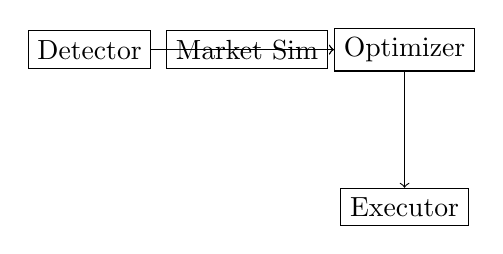
\begin{tikzpicture}[node distance=2cm, auto]
    \node[rectangle, draw] (detect) {Detector};
    \node[rectangle, draw] (market) [right of=detect] {Market Sim};
    \node[rectangle, draw] (opt) [right of=market] {Optimizer};
    \node[rectangle, draw] (exec) [below of=opt] {Executor};
    
    \draw[->] (detect) -- (opt);
    \draw[->] (market) -- (opt);
    \draw[->] (opt) -- (exec);
\end{tikzpicture}
\end{frame}

\begin{frame}
\frametitle{Optimization Algorithm}
\begin{algorithm}[H]
\caption{Triangular Arbitrage Optimization}
\begin{algorithmic}[1]
\Procedure{OptimizeArbitrage}{$\text{opportunities}, \text{constraints}$}
    \State Initialize LP problem
    \State Define decision variables $x_i$ for each opportunity $i$
    \State Set objective function: $\max \sum p_i c_i x_i$
    \For{each constraint type}
        \State Add constraint equations to LP
    \EndFor
    \State Solve LP using simplex method
    \State Extract solution: optimal $x_i^*$ values
    \State Generate execution plan
    \State \Return optimization results
\EndProcedure
\end{algorithmic}
\end{algorithm}
\end{frame}

\begin{frame}
\frametitle{Implementation Technology}
\textbf{Linear Programming Solver}: PuLP (Python)
\begin{itemize}
    \item Uses CBC (Coin-or Branch and Cut) solver
    \item Handles mixed-integer and continuous variables
    \item Interfaces with commercial solvers (CPLEX, Gurobi)
\end{itemize}

\vspace{0.5cm}

\textbf{Data Structures}:
\begin{itemize}
    \item Opportunity objects with profit, confidence, constraints
    \item Portfolio constraint objects with balances, limits
    \item Market condition objects with volatility, liquidity factors
\end{itemize}
\end{frame}

\section{Results and Analysis}

\begin{frame}
\frametitle{Experimental Setup}
\textbf{Test Parameters}:
\begin{itemize}
    \item Portfolio value: \$100,000
    \item Number of opportunities: 15-20 per optimization cycle
    \item Currency pairs: 8 major cryptocurrencies
    \item Risk profiles: Conservative (5-15\%), Moderate (15-35\%), Aggressive (35-60\%)
\end{itemize}

\vspace{0.5cm}

\textbf{Market Simulation}:
\begin{itemize}
    \item Volatility index: 0.2-0.9
    \item Liquidity factors: 0.5-2.0
    \item Transaction fees: 0.08\%-0.4\%
    \item Arbitrage margins: 0.5\%-2.5\%
\end{itemize}
\end{frame}

\begin{frame}
\frametitle{Performance Results}
\begin{table}[h]
\centering
\begin{tabular}{@{}lccc@{}}
\toprule
Risk Profile & Avg Investment & Avg Profit & Avg ROI \\
\midrule
Conservative & \$2,421 & \$35.72 & 1.475\% \\
Moderate & \$13,271 & \$195.77 & 1.475\% \\
Aggressive & \$25,756 & \$379.95 & 1.475\% \\
\bottomrule
\end{tabular}
\caption{Performance by Risk Profile}
\end{table}

\vspace{0.5cm}

\textbf{Key Observations}:
\begin{itemize}
    \item ROI remains consistent across risk profiles
    \item Higher risk tolerance allows larger absolute profits
    \item System successfully respects all constraints
\end{itemize}
\end{frame}

\begin{frame}
\frametitle{Multi-Period Analysis}
\begin{table}[h]
\centering
\begin{tabular}{@{}lccc@{}}
\toprule
Period & Investment & Profit & Cumulative ROI \\
\midrule
1 & \$8,610 & \$156.07 & 1.813\% \\
2 & \$8,597 & \$154.08 & 1.792\% \\
3 & \$8,514 & \$157.96 & 1.855\% \\
\midrule
Total & \$25,721 & \$468.10 & 1.820\% \\
\bottomrule
\end{tabular}
\caption{Three-Period Performance Analysis}
\end{table}

\vspace{0.5cm}

\textbf{Success Rate}: 100\% (all periods found profitable opportunities)
\end{frame}

\begin{frame}
\frametitle{Constraint Analysis}
\textbf{Risk Utilization}:
\begin{itemize}
    \item Average: 26.9\% of risk tolerance
    \item Shows conservative optimization approach
    \item Leaves room for market volatility
\end{itemize}

\vspace{0.5cm}

\textbf{Liquidity Constraints}:
\begin{itemize}
    \item Never exceeded available market depth
    \item Average utilization: 15-20\% of available liquidity
    \item Prevents market impact on execution
\end{itemize}

\vspace{0.5cm}

\textbf{Portfolio Balance}:
\begin{itemize}
    \item All minimum holdings maintained
    \item Diversification across 4-6 currencies
    \item Stable coin allocation: 20-40\% of portfolio
\end{itemize}
\end{frame}

\section{Conclusions and Extensions}

\begin{frame}
\frametitle{Model Advantages}
\textbf{Mathematical Rigor}:
\begin{itemize}
    \item Linear programming guarantees global optimum
    \item Constraint satisfaction ensures feasible solutions
    \item Scalable to large numbers of opportunities
\end{itemize}

\vspace{0.5cm}

\textbf{Practical Benefits}:
\begin{itemize}
    \item Risk management built into optimization
    \item Handles multiple constraints simultaneously
    \item Adaptable to changing market conditions
\end{itemize}

\vspace{0.5cm}

\textbf{Computational Efficiency}:
\begin{itemize}
    \item Linear constraints enable fast solving
    \item Sub-second optimization for 20+ opportunities
    \item Suitable for real-time trading applications
\end{itemize}
\end{frame}

\begin{frame}
\frametitle{Limitations and Assumptions}
\textbf{Model Limitations}:
\begin{itemize}
    \item Linear liquidity consumption approximation
    \item Static profit estimates during optimization
    \item No modeling of execution latency
\end{itemize}

\vspace{0.5cm}

\textbf{Market Assumptions}:
\begin{itemize}
    \item Simultaneous execution of all trades
    \item Perfect information about exchange rates
    \item No regulatory or operational constraints
\end{itemize}

\vspace{0.5cm}

\textbf{Risk Factors}:
\begin{itemize}
    \item Market volatility can eliminate opportunities
    \item Network congestion affects execution speed
    \item Regulatory changes impact market access
\end{itemize}
\end{frame}

\begin{frame}
\frametitle{Future Extensions}
\textbf{Mathematical Enhancements}:
\begin{itemize}
    \item Stochastic programming for uncertainty
    \item Nonlinear constraints for market impact
    \item Multi-objective optimization (profit vs. risk)
\end{itemize}

\vspace{0.5cm}

\textbf{System Improvements}:
\begin{itemize}
    \item Real-time data integration
    \item Machine learning for profit prediction
    \item Dynamic hedging strategies
\end{itemize}

\vspace{0.5cm}

\textbf{Market Extensions}:
\begin{itemize}
    \item Cross-exchange arbitrage
    \item Traditional financial markets
    \item Decentralized finance protocols
\end{itemize}
\end{frame}

\begin{frame}
\frametitle{Practical Implementation Considerations}
\textbf{Real-World Deployment}:
\begin{itemize}
    \item High-frequency data feeds required
    \item Sub-millisecond execution infrastructure
    \item Robust risk monitoring systems
\end{itemize}

\vspace{0.5cm}

\textbf{Regulatory Compliance}:
\begin{itemize}
    \item Know Your Customer (KYC) requirements
    \item Anti-Money Laundering (AML) checks
    \item Reporting and audit trails
\end{itemize}

\vspace{0.5cm}

\textbf{Operational Risk}:
\begin{itemize}
    \item Exchange downtime and connectivity
    \item Wallet security and key management
    \item Market manipulation detection
\end{itemize}
\end{frame}

\begin{frame}
\frametitle{Conclusion}
\textbf{Key Contributions}:
\begin{enumerate}
    \item Formulated triangular arbitrage as linear programming problem
    \item Integrated multiple real-world constraints
    \item Demonstrated consistent profitability with risk management
    \item Provided scalable framework for cryptocurrency trading
\end{enumerate}

\vspace{0.5cm}

\textbf{Academic Value}:
\begin{itemize}
    \item Applies optimization theory to financial markets
    \item Demonstrates constraint modeling techniques
    \item Bridges theoretical mathematics with practical trading
\end{itemize}

\vspace{0.5cm}

\textbf{Industry Relevance}:
\begin{itemize}
    \item Addresses real market inefficiencies
    \item Provides foundation for trading system development
    \item Applicable to various financial instruments
\end{itemize}
\end{frame}

\begin{frame}
\frametitle{Questions and Discussion}
\begin{center}
\Large Thank you for your attention!

\vspace{1cm}

Questions?

\vspace{1cm}

Contact: [Your Email]\\
Code Repository: [GitHub Link]
\end{center}
\end{frame}

\end{document}
